% vim:spell spelllang=fr:
\def\raggedright{}
\documentclass[final,hyperref={pdfpagelabels=false}]{beamer}
%\usepackage{grffile}
%\mode<presentation>{\usetheme{I6dv}}

\usepackage[absolute,overlay]{textpos}
\usepackage[french]{babel}
\usepackage[utf8]{inputenc}
\usepackage[T1]{fontenc}
\usepackage{ae,aecompl}
\usepackage{amsmath,amsthm, amssymb, latexsym}
%\usepackage{figlatex}
\usepackage{multicol}
\usepackage{tikz,url,marvosym,moreverb}
\usetikzlibrary{shapes.geometric}
%\usepackage{times}\usefonttheme{professionalfonts}  % obsolete
%\usefonttheme[onlymath]{serif}
\boldmath


%%% Mon slicing manuel
\let\Coupe=\comment \let\endCoupe=\endcomment
\renewenvironment{Coupe}{   }{   }


% Work around a bug in beamer?
% http://tex.stackexchange.com/questions/4436/beamer-undefined-control-sequence
\providecommand\thispdfpagelabel[1]{}

\setlength{\paperwidth}{20cm}
\setlength{\paperheight}{20cm}
\setlength{\textwidth}{18cm}
\setlength{\textheight}{18cm}
\edef\fontscale{0.5}    % fontscale=(1/sqrt(2))^3

%%%%%%%%%%%%%%%%%%%%%%%%%%%%%%%%%%%%%%%%%%%%%%%
%%%%%%%%%%%%%%%%%%%%%%%%%%%%%%%%%%%%%%%%%%%%%%%
%%%%%%%%%%%%%%%%%%%%%%%%%%%%%%%%%%%%%%%%%%%%%%%
%%%%%%%%%%%%%%%%%%%%%%%%%%%%%%%%%%%%%%%%%%%%%%%
\usepackage{fp}
\edef\myfontscale{1.0}
%% normalize scale depending on poster size
\FPupn{\myfontscale}{myfontscale fontscale * 2 round}
%% scalable vector fonts
\edef\fontSizeX{12}\edef\fontSizeY{14}
\FPupn{\resulttinyX}{myfontscale fontSizeX * 2 round}
\FPupn{\resulttinyY}{myfontscale fontSizeY * 2 round}
\renewcommand*{\tiny}{\fontsize{\resulttinyX}{\resulttinyY}\selectfont}

\edef\fontSizeX{14.4}\edef\fontSizeY{18}
\FPupn{\resultscriptsizeX}{myfontscale fontSizeX * 2 round}
\FPupn{\resultscriptsizeY}{myfontscale fontSizeY * 2 round}
\renewcommand*{\scriptsize}{\fontsize{\resultscriptsizeX}{\resultscriptsizeY}\selectfont}

\edef\fontSizeX{17.28}\edef\fontSizeY{22}
\FPupn{\resultfootnotesizeX}{myfontscale fontSizeX * 2 round}
\FPupn{\resultfootnotesizeY}{myfontscale fontSizeY * 2 round}
\renewcommand*{\footnotesize}{\fontsize{\resultfootnotesizeX}{\resultfootnotesizeY}\selectfont}

\edef\fontSizeX{20.74}\edef\fontSizeY{25}
\FPupn{\resultsmallX}{myfontscale fontSizeX * 2 round}
\FPupn{\resultsmallY}{myfontscale fontSizeY * 2 round}
\renewcommand*{\small}{\fontsize{\resultsmallX}{\resultsmallY}\selectfont}

\edef\fontSizeX{24.88}\edef\fontSizeY{30}
\FPupn{\resultnormalsizeX}{myfontscale fontSizeX * 2 round}
\FPupn{\resultnormalsizeY}{myfontscale fontSizeY * 2 round}
\renewcommand*{\normalsize}{\fontsize{\resultnormalsizeX}{\resultnormalsizeY}\selectfont}

\edef\fontSizeX{29.86}\edef\fontSizeY{37}
\FPupn{\resultlargeX}{myfontscale fontSizeX * 2 round}
\FPupn{\resultlargeY}{myfontscale fontSizeY * 2 round}
\renewcommand*{\large}{\fontsize{\resultlargeX}{\resultlargeY}\selectfont}

\edef\fontSizeX{35.83}\edef\fontSizeY{45}
\FPupn{\resultLargeX}{myfontscale fontSizeX * 2 round}
\FPupn{\resultLargeY}{myfontscale fontSizeY * 2 round}
\renewcommand*{\Large}{\fontsize{\resultLargeX}{\resultLargeY}\selectfont}

\edef\fontSizeX{43}\edef\fontSizeY{54}
\FPupn{\resultLARGEX}{myfontscale fontSizeX * 2 round}
\FPupn{\resultLARGEY}{myfontscale fontSizeY * 2 round}
\renewcommand*{\LARGE}{\fontsize{\resultLARGEX}{\resultLARGEY}\selectfont}

\edef\fontSizeX{51.6}\edef\fontSizeY{64}
\FPupn{\resulthugeX}{myfontscale fontSizeX * 2 round}
\FPupn{\resulthugeY}{myfontscale fontSizeY * 2 round}
\renewcommand*{\huge}{\fontsize{\resulthugeX}{\resulthugeY}\selectfont}

\edef\fontSizeX{61.92}\edef\fontSizeY{77}
\FPupn{\resultHugeX}{myfontscale fontSizeX * 2 round}
\FPupn{\resultHugeY}{myfontscale fontSizeY * 2 round}
\renewcommand*{\Huge}{\fontsize{\resultHugeX}{\resultHugeY}\selectfont}

\edef\fontSizeX{74.3}\edef\fontSizeY{93}
\FPupn{\resultveryHugeX}{myfontscale fontSizeX * 2 round}
\FPupn{\resultveryHugeY}{myfontscale fontSizeY * 2 round}
\newcommand*{\veryHuge}{\fontsize{\resultveryHugeX}{\resultveryHugeY}\selectfont}

\edef\fontSizeX{89.16}\edef\fontSizeY{112}
\FPupn{\resultVeryHugeX}{myfontscale fontSizeX * 2 round}
\FPupn{\resultVeryHugeY}{myfontscale fontSizeY * 2 round}
\newcommand*{\VeryHuge}{\fontsize{\resultVeryHugeX}{\resultVeryHugeY}\selectfont}

\edef\fontSizeX{107}\edef\fontSizeY{134}
\FPupn{\resultVERYHugeX}{myfontscale fontSizeX * 2 round}
\FPupn{\resultVERYHugeY}{myfontscale fontSizeY * 2 round}
\newcommand*{\VERYHuge}{\fontsize{\resultVERYHugeX}{\resultVERYHugeY}\selectfont}

% set the normalfont (default)
\renewcommand*{\normalfont}{\normalsize}

%%%%%%%%%%%%%%%%%%%%%%%%%%%%%%%%%%%%%%%%%%%%%%%
%%%%%%%%%%%%%%%%%%%%%%%%%%%%%%%%%%%%%%%%%%%%%%%
%%%%%%%%%%%%%%%%%%%%%%%%%%%%%%%%%%%%%%%%%%%%%%%
%%%%%%%%%%%%%%%%%%%%%%%%%%%%%%%%%%%%%%%%%%%%%%%

%%%
%%% No navigation, thanks
%%%
\usenavigationsymbolstemplate{}

%\beamertemplategridbackground[1cm]

%\usepackage{snapshot} % will write a .dep file with all dependencies, allows for easy bundling

\usepackage{array,booktabs,tabularx}
\newcolumntype{Z}{>{\centering\arraybackslash}X} % centered tabularx columns
\newcommand{\pphantom}{\textcolor{ta3aluminium}} % phantom introduces a vertical space in p formatted table columns??!!

\listfiles

%%%%%%%%%%%%%%%%%%%%%%%%%%%%%%%%%%%%%%%%%%%%%%%%%%%%%%%%%%%%%%%%%%%%%%%%%%%%%%%%%%%%%%
\graphicspath{{figures/}}

\begin{document}
\begin{Coupe}
\begin{frame}{}
  \begin{textblock*}{50mm}[1,1](61mm,195mm)
    
\includegraphics[height=4\baselineskip]{img/pseudo_logo_CSIRL.pdf}
  \end{textblock*}

  \begin{textblock*}{7cm}[0,1](67.6mm,190mm)
    \vbox{\structure{\LARGE CS IRL}

    \medskip
    {\large Computer Science In Real Life}}
  \end{textblock*}


  \begin{center}
    \structure{\Huge Les algorithmes}

    \bigskip
    \bigskip
    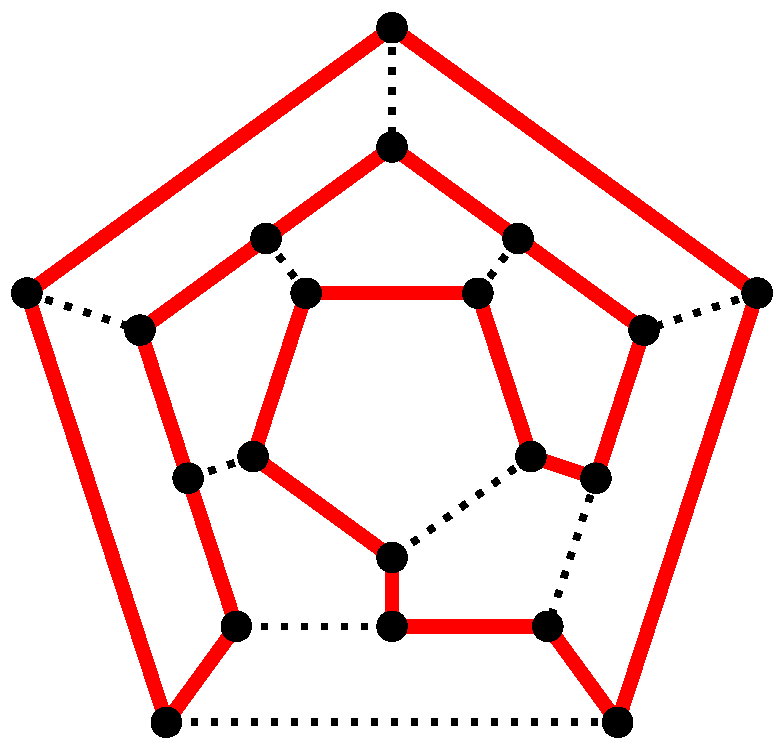
\includegraphics[width=.7\linewidth]{img/Hamiltonian_path.pdf}\label{img:hamiltonian}
    \vspace{5\baselineskip}


    ~

  \end{center}

  
\end{frame}

%%%%%%%%%%%%%%%%%%%%%%%%%%%%%%%%%%%%%%%%%%%%%%%%%%%%%%%%%%%%%%%%%%%%%%%%%%%%%%%%%%%%%%%% 
\begin{frame}
  \vspace{20\baselineskip}
  \vfill
  \begin{block}{À propos de ce document}
    \begin{itemize}
    \item \copyright\ 2011-2012 membres du projet CS IRL. Tous droits réservés.

    \item CS IRL est un \alert{projet libre et ouvert}: vous pouvez copier et
      modifier librement les ressources de ce projet sous les conditions
      données par la CC-BY-SA (en bref, vous pouvez diffuser et modifier ces
      ressources à condition que vous donniez les mêmes droits aux utilisateurs
      de vos copies).
    \item La page web du projet est ici: \url{http://wiki.nybi.cc/index.php/CSIRL}
    \item Les sources des ressources du projet sont entre autres ici: \url{http://github.com/jcb/CSIRL}
    \item Si vous le souhaitez, vous pouvez nous joindre ici: \url{discussions@listes.nybi.cc}
    \end{itemize}
  \end{block}

  \begin{block}{\normalsize Crédits image}\footnotesize
    P\pageref{img:hamiltonian}: Chemin hamiltonien par Ch. Sommer,
    licence GFDL/CC-BY-SA
    \url{http://en.wikipedia.org/wiki/File:Hamiltonian_path.svg}

    P\pageref{img:CSmajor}: Computer Science Major: CC-BY-NC
    \url{http://abstrusegoose.com/206}

%    P\pageref{img:realprog}: Real programmers: \alert{Dessin non libre, à refaire.}
%    \url{http://www.ninisworld.com/oddsends/justforfun/50realprogrammers.html}

    P\pageref{img:electric:city}: Electric City par Mathias M, licence CC-BY-SA
    \url{http://www.flickr.com/photos/mathias_m/342535332/}
  \end{block}
\end{frame}
%%%%%%%%%%%%%%%%%%%%%%%%%%%%%%%%%%%%%%%%%%%%%%%%%%%%%%%%%%%%%%%%%%%%%%%%%%%%%%%%%%%%%%%%
\begin{frame}{Computer Science IRL -- Informatique sans ordinateur\\[-5pt]
  {\large Présentation du projet}}

% Contrairement à ce que beaucoup de monde pense, les ordinateurs ne sont pas la
% seule raison d'être de l'informatique. Pour preuve, ce projet développe
% diverses activités à faire avec des pions, des jetons ou des bouts de bois,
% mais sans aucun ordinateur et même sans électricité. Pourtant, ces petits jeux
% permettront à chacun de découvrir de manière ludique les notions au cœur de
% l'informatique: ce qu'est un algorithme et qu'est ce qui fait qu'un algorithme
% est meilleur qu'un autre, ou encore comment coder et transmettre une
% information.


  \begin{block}{CS IRL? Qu'est ce que c'est?}
    \begin{itemize}
    \item Des activités présentant les bases de l'informatique, mais sans
      ordinateur
    \item Pour chaque activité, un support matériel est proposé pour permettre
      d'\textit{apprendre avec les mains}
    \item Les activités sont rangées en séances cohérentes et progressives
%    \item C'est un projet libre, que vous pouvez télécharger, améliorer et
%      diffuser librement
    \item[
\includegraphics{img/rightpointing_magnifying_glass.pdf}]
      Computer Science In Real Life: Computer Science est la science
      informatique en anglais, tandis que IRL est l'abréviation utilisée sur
      internet pour décrire la vraie vie, ce qui n'est pas sur internet.
    \end{itemize}
  \end{block}

  \begin{block}{Les séances existantes dans la série}
    \begin{itemize}
    \item \structure{Les algorithmes:} Qu'est ce qu'un algorithme? Et une
      heuristique? À quoi ça sert?
    \item \structure{Codes et représentations:} Comment les ordinateurs codent
      et manipulent les données \textit{(à venir)}
    \item \structure{Turzzle:} puzzle de programmation sans ordinateur 
      \textit{(à venir)}
    \end{itemize}
  \end{block}
  \vspace{2\baselineskip}

  \begin{block}{Objectif de la séance algorithmique}
    \begin{itemize}
    \item Expliquer ce qu'est un algorithme et à quoi ça sert quand on veut
      utiliser un ordinateur
    \item Montrer un aspect du travail d'un informaticien, et de celui d'un
      chercheur en informatique
    \item La durée envisagée est d'une heure et demi ou deux heures.
    \item Ce n'est donc pas un cours complet sur l'algorithmique, qui nécessite
      25 à 50h au minimum.\\
      Cours pour aller plus loin (en 48h):
      \url{http://www.loria.fr/~quinson/Teaching/TOP/}
    \item[
\includegraphics{img/rightpointing_magnifying_glass.pdf}]
      Si vous êtes l'animateur, vous trouverez des conseils et des astuces dans le coin de l'animateur en page~\pageref{coin::animateur}.
    \end{itemize}
  \end{block}

  \begin{block}{Matériel nécessaire pour cette séance}
    \begin{itemize}
    \item Des clous, dont un coloré
    \item Des petites planches de tailles différentes
    \item Des legos: cinq couleurs, avec à chaque fois deux pièces $2\times2$ et une
      pièce $4\times2$
    \item Une planche avec des clous plantés (mais qui dépassent); Une cordelette et un marqueur
    \end{itemize}
  \end{block}
\end{frame}
%%%%%%%%%%%%%%%%%%%%%%%%%%%%%%%%%%%%%%%%%%%%%%%%%%%%%%%%%%%%%%%%%%%%%%%%%%%%%%%%%%%%%%%%%%
\begin{frame}{Computer Science IRL -- La séance algorithmique}
  \begin{block}{Introduction: les principales caractéristiques d'un ordinateur}
    \begin{itemize}\vspace{-.2\baselineskip}
    \item \structure{Il est très \alert{rapide}:} il peut calculer de 1 à 1
      million en moins d'une seconde
    \item \structure{Il est parfaitement \alert{obéissant}:} il fait
    tout le temps exactement ce qu'on lui demande
    \item \structure{Il est absolument \alert{stupide}:} il exécute les
      ordres qu'on lui donne, sans la moindre capacité d'initiative.
      \begin{itemize}\vspace{-.8\baselineskip}
      \item Par exemple, si on demande à un ordinateur de s'arrêter, il le fait\ldots
      \item Autre exemple, quand j'indique à des amis comment venir chez moi,
        je leur donne des indications comme "troisième à droite" ou "à gauche
        au 2ieme feu". Si je me trompe dans mes indications ("à gauche" au lieu
        de "à droite") et que cela les ferait prendre l'autoroute à
        contre-sens, mes amis vont faire preuve de sens commun et ne pas
        appliquer la consigne. Les ordinateurs n'ont \textbf{aucun} sens commun.
      \item Bug (n.m.): consigne erronée donnée par un humain et appliquée bêtement par une machine.

      \end{itemize}

    \end{itemize}
  \end{block}\vspace{-.5\baselineskip}

  \begin{block}{Le travail d'un informaticien}
    \begin{itemize}\vspace{-.2\baselineskip}
    \item Se faire obéir d'un serviteur aussi stupide qu'un tas de fil demande
      un peu d'organisation
    \item Pour décomposer suffisamment les tâches à réaliser, il réfléchit à
      \textbf{comment} faire\\
      {\small (un peu comme un cycliste qui descendrait du vélo pour se regarder
        pédaler afin d'expliquer ensuite comment faire)}
    \item Pour chaque problème, il faut d'abord définir:
      \begin{itemize}
      \item \structure{la situation initiale:} le point de départ du problème
      \item \structure{les opérations possibles:} ce que j'ai le droit de faire pour faire
        évoluer la situation
      \item \structure{la situation finale:} ce vers quoi je veux tendre, l'état
        du problème quand je l'ai résolu
      \end{itemize}
    \end{itemize}
  \end{block}


  \centerline{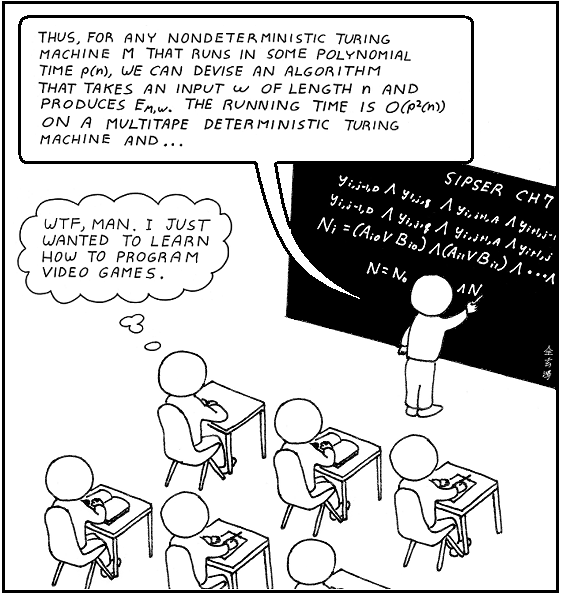
\includegraphics[width=.4\linewidth]{img/computer_science_major.PNG}\label{img:CSmajor}}
\end{frame}
%%%%%%%%%%%%%%%%%%%%%%%%%%%%%%%%%%%%%%%%%%%%%%%%%%%%%%%%%%%%%%%%%%%%%%%%%%%%%%%%%%%%%%%%
%%%%%%%%%%%%%%%%%%%%%%%%%%%%%%%%%%%%%%%%%%%%%%%%%%%%%%%%%%%%%%%%%%%%%%%%%%%%%%%%%%%%%%%%
%%%%%%%%%%                          LE JEU DE NIM
%%%%%%%%%%%%%%%%%%%%%%%%%%%%%%%%%%%%%%%%%%%%%%%%%%%%%%%%%%%%%%%%%%%%%%%%%%%%%%%%%%%%%%%%
%%%%%%%%%%%%%%%%%%%%%%%%%%%%%%%%%%%%%%%%%%%%%%%%%%%%%%%%%%%%%%%%%%%%%%%%%%%%%%%%%%%%%%%%
\newcommand{\clou}[3]{\draw[#3,line width=2pt] (.5*#1,.6*#2) -- +(.3,0) --  +(.15,0) -- +(.15,.5);}
\newcommand{\clous}[2]{\foreach \x/\y in {#2} {\clou{\x}{\y}{#1}}}

\begin{frame}{Activité: le jeu de Nim}

  Voici un premier petit jeu simple, pour rentrer dans le sujet.

  \begin{block}{Matériel}
    \begin{itemize}
    \item 15 clous identiques
    \item 1 clou différencié (ou une vis)
    \end{itemize}
  \end{block}

  \begin{block}{Règle du jeu}
    \begin{itemize}
    \item Chaque joueur prend tour à tour soit 1 soit 2 soit 3 clous
    \item Celui qui prend le dernier clou a gagné
    \end{itemize}
  \end{block}

  \bigskip\bigskip
  \centerline{
    \begin{frame}{Activité: le jeu de Nim}

  Voici un premier petit jeu simple, pour rentrer dans le sujet.

  \begin{block}{Matériel}
    \begin{itemize}
    \item 16 petits objets (clous, allumettes, boulettes de papier ... peu importe !)
    \end{itemize}
  \end{block}

  \begin{block}{Règle du jeu}
    \begin{itemize}
    \item Disposer les 16 objets sur une table
    \item Les deux joueurs prennent tour à tour 1, 2 ou 3 objets
    \item Le joueur qui prend le dernier objet à gagné
    \end{itemize}
  \end{block}

  \bigskip \bigskip  \bigskip \bigskip

  \begin{center}
    % rendre l'illustration plus utile en la transformant en exemple de partie?
    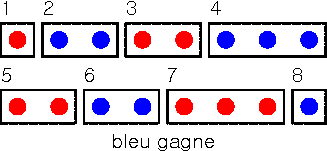
\includegraphics[width=0.8\linewidth]{img/nim.pdf}
  \end{center}

\end{frame}

\begin{frame}{Ce qu'il faut retenir du jeu de Nim}

  \begin{block}{L'intérêt majeur de ce jeu est qu'il est sans suspense 
      {\color{black}\normalsize(voire, sans intérêt ;)}}
    \begin{itemize}
    \item Celui qui commence (\structure{J1}) perd, car il existe un truc pour
      que \structure{J2} gagne à tous les coups
    \item \structure{Stratégie gagnante:} Laisser 4, 8, 12 ou 16 objets à
      l'adversaire (un multiple de 4)
    \end{itemize}
  \end{block}

  \begin{columns}
    \begin{column}{0.7\linewidth}

      \begin{block}{Se convaincre de l'efficacité de la stratégie gagnante}
        Prenons le dernier tour comme exemple. Il reste 4 objets, et J1 joue.

        \begin{itemize}
        \item Si J1 prend \alert{1} objet, J2 en prend \structure{3} (dont le dernier) 
        \item Si J1 prend \alert{2} objets, J2 en prend \structure{2} (dont le dernier)
        \item Si J1 prend \alert{3} objets, J2 en prend \structure{1} (le dernier) 
        \end{itemize}        
        %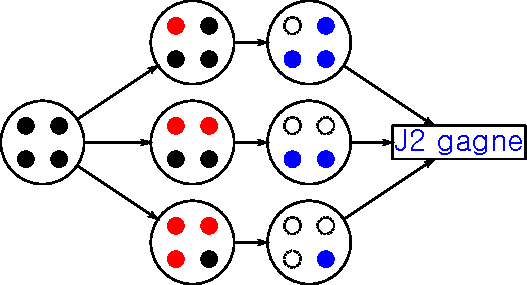
\includegraphics[width=0.6\linewidth]{img/nim4.pdf}

        Dans ce cas, si J2 sait jouer, J1 perd à tous les coups.  En appliquant la même méthode, J2 peut guider le jeu de manière à passer de 16 objets à 12, puis 8 et enfin 4. Donc, si J2 sait jouer, J1 a perdu la partie avant même de commencer.
        
        \center{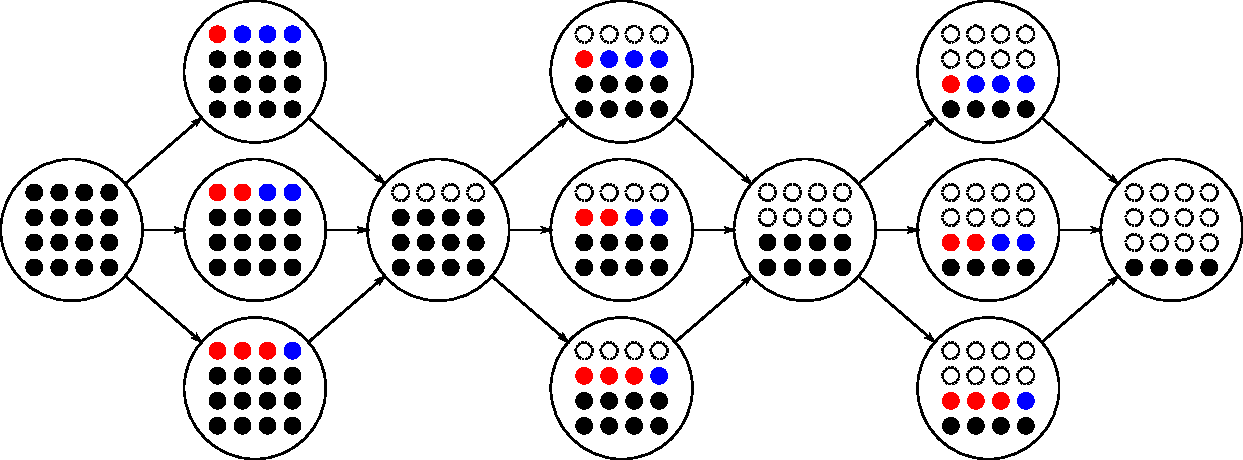
\includegraphics[width=\linewidth]{img/nim16.pdf}}
      \end{block}

    \end{column}
    \begin{column}{0.3\linewidth}

      \begin{block}{Pour aller plus loin}
        On pourrait imaginer un cas plus général du jeu de Nim :

        \begin{itemize}
          \item Il y a $N$ objets sur la table au début du jeu (pour notre version, $N=16$)
          \item Un joueur peut prendre jusqu'à $X$ objets à la fois (pour notre version, $X=3$)
        \end{itemize}

        Quelles modifications doit-on apporter à notre stratégie gagnante pour qu'elle marche dans le cas général ?
      \end{block}

    \end{column}
  \end{columns}

  \begin{block}{Le rapport avec l'informatique}
    \begin{itemize}
    \item Passer de la situation initiale à la situation finale à coup sûr demande d'avoir
      une \textit{stratégie gagnante}
    \item C'est un \alert{\textbf{algorithme}} en informatique, une recette de
      cuisine ou un manuel de montage de meubles
    \item Pour se faire obéir du tas de fils, l'informaticien cherche
      l'algorithme pour résoudre le problème,\\
      puis il écrit le \alert{\textbf{programme}} (traduction de l'algorithme
      dans un langage informatique)
    \end{itemize}
  \end{block}

\end{frame}

  }


\end{frame}
%%%%%%%%%%%%%%%%%%%%%%%%%%%%%%%%%%%%%%%%%%%%%%%%%%%%%%%%%%%%%%%%%%%%%%%%%%%%%%%%%%%%%%%%%%%%

\begin{frame}{Ce qu'il faut retenir du jeu de Nim}

  \begin{block}{L'intérêt majeur de ce jeu est qu'il est sans suspense 
      {\color{black}\normalsize(voire, sans intérêt ;)}}
    \begin{itemize}
    \item Celui qui commence (\structure{J1}) perd, car il existe un truc pour
      que \structure{J2} gagne à tous les coups
    \item \structure{Stratégie gagnante:} Laisser 4, 8, 12 ou 16 clous à
      l'adversaire (un multiple de 4)
    \end{itemize}
  \end{block}

  \begin{block}{Se convaincre de l'efficacité de la stratégie gagnante}
    Prenons le dernier tour comme exemple. Il reste 4 clous, et J1 joue.

    \vspace{-\baselineskip}
    \begin{columns}
      \begin{column}{.55\linewidth}
        \begin{itemize}
        \item Si J1 prend \alert{1} clou, J2 en prend \structure{3} (dont le dernier) 
        \item Si J1 prend \alert{2} clous, J2 en prend \structure{2} (dont le dernier)
        \item Si J1 prend \alert{3} clous, J2 en prend \structure{1} (le dernier) 
        \end{itemize}        
      \end{column}      
      \begin{column}{.35\linewidth}
        \begin{tikzpicture}[
  scale=0.5,
  board/.style={ellipse,inner sep=0pt,minimum width=2cm,minimum height=1.6\baselineskip,draw=black}]

  \node[board] (init) at (0,0) {~};
  \clous{shift=(init),draw=black}{ 0/.4, -1/-.6,0/-.6,1/-.6}

  \node[board] (A1)   at (5,2) {~};
  \node[board] (A2)   at (5,0) {~};
  \node[board] (A3)   at (5,-2) {~};
  \node[board] (B)   at  (10,0) {J2 gagne};
  \pgfkeys{/pgf/number format/.cd,fixed,precision=0}
  \foreach \b in {1,2,3} {
    \draw[->] (init) --  (A\b)  node[above,midway] {\color{red}\pgfmathint{\b}\pgfmathresult} ;
    \draw[->] (A\b) -- (B) node[above,midway] {\color{blue}\pgfmathint{3-\b+1}\pgfmathresult} ;
  }
  \clous{shift=(A1),draw=blue}{ 0/.4, -1/-.6,0/-.6}
  \clous{shift=(A1),draw=red}{1/-.6}

  \clous{shift=(A2),draw=blue}{ 0/.4, -1/-.6}
  \clous{shift=(A2),draw=red}{0/-.6,1/-.6}

  \clous{shift=(A3),draw=blue}{ 0/.4}
  \clous{shift=(A3),draw=red}{-1/-.6,0/-.6,1/-.6}
\end{tikzpicture}        

      \end{column}
    \end{columns}

    \vspace{-.5\baselineskip}
    Quoi qu'il fasse, J1 a donc perdu dans ce cas, si J2 sait jouer. \\[\baselineskip]
    De plus, J2 peut ammener J1 dans cette situation à coup sûr:
    \begin{tikzpicture}[
  scale=0.5,
  board/.style={circle,inner sep=0pt,minimum size=2cm,draw=black}]

  \node[board] (init) at (0,0) {};
  \clous{shift=(init),draw=black}{
                -1/ 1,0/ 1,1/ 1,
          -2/ 0,-1/-0,0/ 0,1/ 0,2/0,
    -3/-1,-2/-1,-1/-1,0/-1,1/-1,2/-1,3/-1}
  \clous{shift=(init),draw=black!3!red!15!yellow}{ 0/ 2}

  \node[board] (A1)   at (5,4) {};
  \node[board] (A2)   at (5,0) {};
  \node[board] (A3)   at (5,-4) {};
  \node[board] (B)   at  (10,0) {};
  \node[board] (C1)   at (15,4) {};
  \node[board] (C2)   at (15,0) {};
  \node[board] (C3)   at (15,-4) {};
  \node[board] (D)   at  (20,0) {};

  \node[board] (E1)   at (25,4) {};
  \node[board] (E2)   at (25,0) {};
  \node[board] (E3)   at (25,-4) {};
  \node[board] (F)   at  (30,0) {};
  \pgfkeys{/pgf/number format/.cd,fixed,precision=0}
  \foreach \b in {1,2,3} {
    \draw[->] (init) --  (A\b)  node[above,midway] {\color{red}\pgfmathint{\b}\pgfmathresult} ;
    \draw[->] (A\b) -- (B) node[above,midway] {\color{blue}\pgfmathint{3-\b+1}\pgfmathresult} ;

    \draw[->] (B) --  (C\b)  node[above,midway] {\color{red}\pgfmathint{\b}\pgfmathresult} ;
    \draw[->] (C\b) -- (D) node[above,midway] {\color{blue}\pgfmathint{3-\b+1}\pgfmathresult} ;

    \draw[->] (D) --  (E\b)  node[above,midway] {\color{red}\pgfmathint{\b}\pgfmathresult} ;
    \draw[->] (E\b) -- (F) node[above,midway] {\color{blue}\pgfmathint{3-\b+1}\pgfmathresult} ;
    \clous{shift=(A\b),draw=black}{
                        0/2,
                  -1/ 1,0/ 1,1/ 1,
            -2/ 0,-1/-0,0/ 0,1/ 0,2/0,
      -3/-1,-2/-1,-1/-1}

    \clous{shift=(C\b),draw=black}{
                        0/2,
                  -1/ 1,0/ 1,1/ 1,
            -2/ 0,-1/-0,0/ 0,1/ 0}

    \clous{shift=(E\b),draw=black}{
                        0/2,
                  -1/ 1,0/ 1,1/ 1}
  }
  \clous{shift=(A1),draw=red}{ 3/-1}
  \clous{shift=(A1),draw=blue}{0/-1,1/-1,2/-1}
  \clous{shift=(A2),draw=red}{2/-1,3/-1}
  \clous{shift=(A2),draw=blue}{0/-1,1/-1}
  \clous{shift=(A3),draw=red}{1/-1,2/-1,3/-1}
  \clous{shift=(A3),draw=blue}{0/-1}

  \clous{shift=(C1),draw=red}{-1/-1}
  \clous{shift=(C1),draw=blue}{2/0,-3/-1,-2/-1}
  \clous{shift=(C2),draw=red}{-2/-1,-1/-1}
  \clous{shift=(C2),draw=blue}{2/0,-3/-1}
  \clous{shift=(C3),draw=red}{-3/-1,-2/-1,-1/-1}
  \clous{shift=(C3),draw=blue}{2/0}

  \clous{shift=(E1),draw=red}{1/ 0}
  \clous{shift=(E1),draw=blue}{-2/ 0,-1/-0,0/ 0}
  \clous{shift=(E2),draw=red}{0/ 0,1/ 0}
  \clous{shift=(E2),draw=blue}{-2/ 0,-1/-0}
  \clous{shift=(E3),draw=red}{-1/-0,0/ 0,1/ 0}
  \clous{shift=(E3),draw=blue}{-2/ 0}

  \clous{shift=(B),draw=black}{
                        0/2,
                  -1/ 1,0/ 1,1/ 1,
            -2/ 0,-1/-0,0/ 0,1/ 0,2/0,
      -3/-1,-2/-1,-1/-1}
  \clous{shift=(D),draw=black}{
                        0/2,
                  -1/ 1,0/ 1,1/ 1,
            -2/ 0,-1/-0,0/ 0,1/ 0}
  \clous{shift=(F),draw=black}{
                        0/2,
                  -1/ 1,0/ 1,1/ 1}
\end{tikzpicture}

    Donc J1 a perdu avant de commencer.
  \end{block}

  \begin{block}{Le rapport avec l'informatique}
    \begin{itemize}
    \item Passer de la situation initiale à la situation finale à coup sûr demande d'avoir
      une \textit{stratégie gagnante}
    \item C'est un \alert{\textbf{algorithme}} en informatique, une recette de
      cuisine ou un manuel de montage de meubles
    \item Pour se faire obéir du tas de fils, l'informaticien cherche
      l'algorithme pour résoudre le problème,\\
      puis il écrit le \alert{\textbf{programme}} (traduction de l'algorithme
      dans un langage informatique)
    \end{itemize}
  \end{block}
\end{frame}
%%%%%%%%%%%%%%%%%%%%%%%%%%%%%%%%%%%%%%%%%%%%%%%%%%%%%%%%%%%%%%%%%%%%%%%%%%%%%%%%%%%%%%%%%
%%%%%%%%%%%%%%%%%%%%%%%%%%%%%%%%%%%%%%%%%%%%%%%%%%%%%%%%%%%%%%%%%%%%%%%%%%%%%%%%%%%%%%%%%
%%%%%%%%%%%%%%% LE JEU DU CRÊPIER
%%%%%%%%%%%%%%%%%%%%%%%%%%%%%%%%%%%%%%%%%%%%%%%%%%%%%%%%%%%%%%%%%%%%%%%%%%%%%%%%%%%%%%%%%
%%%%%%%%%%%%%%%%%%%%%%%%%%%%%%%%%%%%%%%%%%%%%%%%%%%%%%%%%%%%%%%%%%%%%%%%%%%%%%%%%%%%%%%%%
\begin{frame}{Activité: Le crêpier psycho-rigide}

  \begin{block}{Matériel}
    \begin{itemize}
    \item des planchettes en bois de tailles et de couleurs différentes (faces reconnaissables)
    \item éventuellement une pelle à tarte pour retourner les planchettes
    \end{itemize}
  \end{block}

  \begin{block}{Règle du jeu}
    \begin{itemize}
    \item Le crêpier doit ranger ses crêpes de la plus grande à la plus petite,
      face colorée vers le haut
    \item il peut retourner une ou plusieurs crêpes à la fois
    \item l'ordre des crêpes ne peut pas être modifié au moment de retourner
      une pile
    \end{itemize}
  \end{block}
%  mettre une illustration ici ?

\end{frame}
%%%%%%%%%%%%%%%%%%%%%%%%%%%%%%%%%%%%%%%%%%%%%%%%%%%%%%%%%%%%%%%%%%%%%%%%%%%%%%%%%%%%%%%%%
\begin{frame}{Ce qu'il faut retenir du  crêpier psycho-rigide}

  \begin{block}{Un algorithme}
    \begin{itemize}
    \item n'a d'intérêt que si on peut l'expliquer
    \item doit être suffisamment simple pour pouvoir l'expliquer à une machine
    \item \alert{\textbf{«Diviser pour mieux régner»}} : on essaie
    toujours de décomposer un algorithme en tâches simples
    \end{itemize}
  \end{block}

  \begin{block}{L'algorithme que doit suivre le crêpier est :}
    \begin{itemize}
    \item ramener la plus grande crêpe en haut de la pile
    \item retourner pour que la face brûlée soit vers le haut
    \item retourner la pile de sorte à mettre la plus grande crêpe en bas
    \item réitérer avec la crêpe de taille inférieure
    \end{itemize}
  \end{block}

  \begin{block}{Le rapport avec l'informatique}
    \begin{itemize}
    \item l'informaticien passe son temps à trouver des algorithmes et  à les
    expliquer à la machine
    \item le principe \alert{\textbf{«Diviser pour mieux régner»}} est
    fondamental en informatique
    \end{itemize}
  \end{block}
\end{frame}
%%%%%%%%%%%%%%%%%%%%%%%%%%%%%%%%%%%%%%%%%%%%%%%%%%%%%%%%%%%%%%%%%%%%%%%%%%%%%%%%%%%%%%%%%
%%%%%%%%%%%%%%%%%%%%%%%%%%%%%%%%%%%%%%%%%%%%%%%%%%%%%%%%%%%%%%%%%%%%%%%%%%%%%%%%%%%%%%%%%
%%%%%%%%%%%%%%%%%   LES BONSHOMMES
%%%%%%%%%%%%%%%%%%%%%%%%%%%%%%%%%%%%%%%%%%%%%%%%%%%%%%%%%%%%%%%%%%%%%%%%%%%%%%%%%%%%%%%%%
%%%%%%%%%%%%%%%%%%%%%%%%%%%%%%%%%%%%%%%%%%%%%%%%%%%%%%%%%%%%%%%%%%%%%%%%%%%%%%%%%%%%%%%%%

\newcommand{\maisonPair}[5]{ \begin{tikzpicture}
  \node[name=m,shape=regular polygon,regular polygon sides=#3,minimum size=22mm,rotate=(360/#3)]{};
  \node[name=b,shape=regular polygon,regular polygon sides=#4,minimum size=14mm,rotate=(360/#4)/2]{};
  \foreach \base/\maison in {#5} {
    \draw[shift=(m.corner \base)]
       node[shape=ellipse,fill=\maison,draw=black,rotate=((360/#3)*(\base-1))+(360/#3/2)] {~~};
  }
  \foreach \bb in {1,...,#4} {
    \draw[shift=(b.corner \bb)] node[name=bb \bb]{};
  }
  \foreach \base/\maison in {#1} {
    \draw[shift=(b.corner \base)]
       node[name=bb \base,shape=circle,fill=\maison,draw=black,inner sep=.1]
       {~~~};
%         {\footnotesize\base};
  }
  #2
\end{tikzpicture} }
\newcommand{\maisonImpair}[5]{ \begin{tikzpicture}
  \node[name=m,shape=regular polygon,regular polygon sides=#3,
        minimum size=22mm, inner sep=0pt]{};
  \node[name=b,shape=regular polygon,regular polygon sides=#4,minimum size=14mm]{};
  \foreach \base/\maison in {#5} {
    \draw[shift=(m.corner \base)]
       node[shape=ellipse,fill=\maison,draw=black,rotate=(360/#3)*(\base-1)] {~~};
  }
  \foreach \base/\maison in {#1} {
    \draw[shift=(b.corner \base)]
       node[shape=circle,fill=\maison,draw=black,inner sep=.1] {~~~};
  }
  \foreach \bb in {1,...,#4} {\draw[shift=(b.corner \bb)] node[name=bb \bb] {};}
%  \foreach \bb in {1,...,#4} {\draw[shift=(b.corner \bb)] node[name=bb \bb]{\tiny\bb};}%debug the bonshommes names
  #2
\end{tikzpicture} }

\newcommand{\maisonQuatre}[2]{\maisonPair{#1}{#2}{4}{12}{1/A,2/B,3/C,4/D}}
\newcommand{\maisonCinq}[2]{\maisonImpair{#1}{#2}{5}{20}{1/A,2/B,3/C,4/D,5/E}}
\newcommand{\maisonSix}[2]{\maisonPair{#1}{#2}{6}{24}{1/A,2/B,3/C,4/D,5/E,6/F}}
\newcommand{\maisonSept}[2]{\maisonImpair{#1}{#2}{7}{28}{1/A,2/B,3/C,4/D,5/E,6/F,7/G}}

\colorlet{A}{green!60}
\colorlet{B}{red!80}
\colorlet{C}{purple!40}
\colorlet{D}{black!2!yellow}
\colorlet{E}{blue!70}
\colorlet{F}{orange!80}
\colorlet{G}{olive}
\colorlet{H}{magenta}
\colorlet{I}{lime}
\colorlet{J}{pink}

\newcommand{\pawn}[1]{\tikz \draw node[shape=circle,fill=#1,draw=black,inner sep=.1] {~~~};}



%%%%%%%%%%%%%%%%%%%%%%%%%%%%%%%%%%%%%%%%%%%%%%%%%%%%%%%%%%%%%%%%%%%%%%%%%%%%%%%%%%%%%%%
\begin{frame}{Activité: Base-ball multicolore}
  \begin{block}{Matériel nécessaire}
    \begin{itemize}
    \item Plusieurs équipes bien différentiables, chacune composée d'une maison
      et de deux bonshommes\\
      (des legos, des bouts de bois, des cailloux, du fil électrique de
      différentes couleurs, ou autres)

    \item Il faut 5 équipes au minimum. 7 équipes sont préférables, et on peut
      en utiliser une dizaine
    \end{itemize}
  \end{block}

  \begin{block}{Règles du jeu (exemple à quatre équipes)}
    \begin{itemize}
    \item \structure{Situation initiale:}~\\
      On place 4 maisons autour du terrain, et on répartit 7 bonshommes au
      hasard dans les maisons\\
     (il manque donc l'un des bonshommes, qui est mis de coté et ne sera
      pas utilisé)
    \item \structure{Coups autorisés:}
      \begin{itemize}\normalsize
      \item On peut déplacer un seul bonhomme à la fois, d'une maison vers une
        maison adjacente\\
        $\leadsto$ il est interdit de traverser le terrain
      \item On ne peut jamais avoir plus de 2 bonshommes par maison\\
        $\leadsto$ on ne peut bouger que d'une maison adjacente vers la maison
        où il y a un trou
      \end{itemize}
    \item  \structure{Situation finale:}
      L'objectif est de ramener tous les bonshommes dans la maison de leur couleur.
    \end{itemize}
  \end{block}

  \vspace{-\baselineskip}
  \begin{columns}
    \begin{column}{.17\linewidth}\center
      \maisonQuatre{2/B,3/A, 5/D, 8/B,9/C, 11/D,12/A} {}

      \structure{Situation initiale}
    \end{column}
    \begin{column}{.17\linewidth}\center
      \maisonQuatre{2/B,3/A, 5/D, 8/B,9/C, 11/D,12/A}
                   {
                     \draw[->,ultra thick,draw=black!10!green] (bb 2) -> (bb 6);
                     \draw[->,ultra thick,draw=black!10!green] (bb 3) -> (bb 6);
                     \draw[->,ultra thick,draw=black!10!green] (bb 9) -> (bb 6);
                     \draw[->,ultra thick,draw=black!10!green] (bb 8) -> (bb 6);}

      \structure{Coups autorisés}
    \end{column}
    \begin{column}{.17\linewidth}\center
      \maisonQuatre{2/B,3/A, 5/D, 8/B,9/C, 11/D,12/A}
                   { \draw[->,ultra thick,draw=red] (bb 11) -> (bb 6);
                     \draw[->,ultra thick,draw=red] (bb 12) -> (bb 6);
                     \draw[->,ultra thick,draw=red] (bb 12) -> (bb 2);
                     \draw[->,ultra thick,draw=red] (bb 2) -> (bb 12);
                     \draw[->,ultra thick,draw=red] (bb 5) -> (bb 3);
                     \draw[->,ultra thick,draw=red] (bb 5)
                        .. controls (0pt,0pt) .. (bb 8);
                     \draw[->,ultra thick,draw=red] (bb 11) -> (bb 9);
                     \draw[->,ultra thick,draw=red] (bb 9) -> (bb 11);
                   }

      \structure{Coups interdits}
    \end{column}
    \begin{column}{.17\linewidth}\center
      \maisonQuatre{2/A,3/A, 5/B,6/B, 8/C,9/C, 11/D}{}

      \structure{Situation finale}
    \end{column}
  \end{columns}

  \bigskip
  \begin{block}{Objectif de l'activité}
    \begin{itemize}
    \item Le plus important n'est pas  de ramener les bonshommes dans leurs
      maisons
    \item L'objectif est d'expliquer comment on fait. On cherche donc
      l'algorithme correspondant
    \item Si on veut utiliser plus de couleurs, c'est possible.
    \end{itemize}
  \end{block}

  \centerline{
    \maisonCinq{1/A,2/A, 5/B,6/B, 9/C,10/C, 13/D,14/D, 17/E}{}
    \maisonSix{2/A,4/A,  6/B,8/B, 10/C,12/C, 14/D,16/D, 18/E,20/E, 22/F}{}
    \maisonSept{1/A,2/A, 5/B,6/B, 9/C,10/C, 13/D,14/D, 17/E,18/E, 21/F,22/F, 25/G}{}
    \maisonPair{2/A,4/A, 6/B,8/B, 10/C,12/C, 14/D,16/D, 18/E,20/E, 22/F,24/F,
      26/G,28/G, 30/H}{}{8}{32}
               {1/A,2/B,3/C,4/D,5/E,6/F,7/G,8/H}
    % Neuf maisons
    \maisonImpair{1/A,2/A, 5/B,6/B, 9/C,10/C, 13/D,14/D, 17/E,18/E,
                  21/F,22/F, 25/G,26/G, 29/H,30/H,  33/I}{}{9}{36}
               {1/A,2/B,3/C,4/D,5/E,6/F,7/G,8/H,9/I}
    % Dix maisons
    \maisonPair{2/A,4/A, 6/B,8/B, 10/C,12/C, 14/D,16/D, 18/E,20/E, 22/F,24/F,
      26/G,28/G, 30/H,32/H, 34/I,36/I, 38/J}{}{10}{40}
               {1/A,2/B,3/C,4/D,5/E,6/F,7/G,8/H,9/I,10/J}
  }


\end{frame}
%%%%%%%%%%%%%%%%%%%%%%%%%%%%%%%%%%%%%%%%%%%%%%%%%%%%%%%%%%%%%%%%%%%%%%%%%%%%%%%%%%%%%%%%%
\newcommand{\flecherond}[1]{
  \draw[ultra thick] (0,0) circle (3mm);
  \draw[ultra thick,rotate=#1*72] (3mm,0) -- +(-.15,-.08);
  \draw[ultra thick,rotate=#1*72] (3mm,0) -- +(.08,-.15);
  \draw[fill=white,draw=white,rotate=#1*72] (3mm,2.5pt) circle (2pt);
}
\begin{frame}{Un premier algorithme pour le base-ball multicolore}
  \begin{block}{L'algorithme}
    \begin{itemize}
    \item On ne s'autorise qu'à tourner dans un seul sens.
    \item On n'a plus 4 coups possibles, mais deux seulement (car 2 bonshommes
      tourneraient à l'envers)
    \item Entre ces deux bonshommes, je déplace celui dont la destination est la
      plus lointaine
    \end{itemize}
  \end{block}


  \begin{block}{Exemple d'exécution}
    \begin{columns}
  % J'avais une case de trop...
  % \begin{column}{.15\linewidth}\center
  %   \maisonCinq{1/D,2/B, 5/A,6/C, 9/E,10/D, 13/A,14/C, 17/B}{\flecherond{0}}\\
  %   {\small $4>2\leadsto$ \pawn{C}}        
  % \end{column}

  \begin{column}{.15\linewidth}\center
    \maisonCinq{1/D,2/B, 5/A,6/C, 9/E,10/D, 13/A, 17/B,18/C}{\flecherond{4}}\\
    {\small $2>1\leadsto$ \pawn{E}}        
  \end{column}

  \begin{column}{.15\linewidth}\center
    \maisonCinq{1/D,2/B, 5/A,6/C, 10/D, 13/A,14/E, 17/B,18/C}{\flecherond{3}}\\
    {\small $4>1\Rightarrow$ \pawn{A}}
  \end{column}

  \begin{column}{.15\linewidth}\center
    \maisonCinq{1/D,2/B, 6/C, 9/A,10/D, 13/A,14/E, 17/B,18/C}{\flecherond{2}}\\
    {\small $3>1\leadsto$ \pawn{D}}        
  \end{column}

  \begin{column}{.15\linewidth}\center
    \maisonCinq{2/B, 5/D,6/C, 9/A,10/D, 13/A,14/E, 17/B,18/C}{\flecherond{1}}\\
    {\small $3>2\leadsto$ \pawn{C}}        
  \end{column}
  \begin{column}{.15\linewidth}\center
    \maisonCinq{1/C,2/B, 5/D,6/C, 9/A,10/D, 13/A,14/E, 17/B}{\flecherond{0}}\\
    {\small $2>1\leadsto$ \pawn{A}}        
  \end{column}
\end{columns}
%%%%%%%%%%%%%
\begin{columns}
  \begin{column}{.15\linewidth}\center
    \maisonCinq{1/C,2/B, 5/D,6/C, 9/A,10/D, 14/E, 17/B,18/A}{\flecherond{4}}\\
    {\small $2>1\leadsto$ \pawn{A}}        
  \end{column}

  \begin{column}{.15\linewidth}\center
    \maisonCinq{1/C,2/B, 5/D,6/C, 10/D, 13/A,14/E, 17/B,18/A}{\flecherond{3}}\\
     {\small $2>1\leadsto$ \pawn{D}}        
  \end{column}

  \begin{column}{.15\linewidth}\center
    \maisonCinq{1/C,2/B, 6/C, 9/D,10/D, 13/A,14/E, 17/B,18/A}{\flecherond{2}}\\
     {\small $2>1\leadsto$ \pawn{C}}        
  \end{column}

  \begin{column}{.15\linewidth}\center
    \maisonCinq{2/B, 5/C,6/C, 9/D,10/D, 13/A,14/E, 17/B,18/A}{\flecherond{1}}\\
     {\small $2>1\leadsto$ \pawn{B}}        
  \end{column}
  \begin{column}{.15\linewidth}\center
    \maisonCinq{1/B,2/B, 5/C,6/C, 9/D,10/D, 13/A,14/E, 18/A}{\flecherond{0}}\\
     {\small $2>1\leadsto$ \pawn{A}}        
  \end{column}
\end{columns}
%%%%%%%%%%%%%
\begin{columns}
  \begin{column}{.15\linewidth}\center
    \maisonCinq{1/B,2/B, 5/C,6/C, 9/D,10/D, 14/E, 17/A,18/A}{\flecherond{4}}\\
     {\small $1=1\leadsto$ \pawn{D}}        
  \end{column}

  \begin{column}{.15\linewidth}\center
    \maisonCinq{1/B,2/B, 5/C,6/C, 10/D, 13/D,14/E, 17/A,18/A}{\flecherond{3}}\\
     {\small $1=1\leadsto$ \pawn{C}}        
  \end{column}

  \begin{column}{.15\linewidth}\center
    \maisonCinq{1/B,2/B, 6/C, 9/C,10/D, 13/D,14/E, 17/A,18/A}{\flecherond{2}}\\
     {\small $1=1\leadsto$ \pawn{B}}        
  \end{column}

  \begin{column}{.15\linewidth}\center
    \maisonCinq{2/B, 5/B,6/C, 9/C,10/D, 13/D,14/E, 17/A,18/A}{\flecherond{1}}\\
     {\small $1=1\leadsto$ \pawn{A}}        
  \end{column}

  \begin{column}{.15\linewidth}\center
    \maisonCinq{1/A,2/B, 5/B,6/C, 9/C,10/D, 13/D,14/E, 18/A}{\flecherond{0}}\\
     {\small $1>0\leadsto$ \pawn{E}}        
  \end{column}
\end{columns}
%%%%%%%%%%%%%
\begin{columns}[t]
  \begin{column}{.15\linewidth}\center
    \maisonCinq{1/A,2/B, 5/B,6/C, 9/C,10/D, 13/D, 17/E,18/A}{\flecherond{4}}\\
     {\small $1>0\leadsto$ \pawn{D}}
  \end{column}

  \begin{column}{.15\linewidth}\center
    \maisonCinq{1/A,2/B, 5/B,6/C, 9/C, 13/D,14/D, 17/E,18/A}{\flecherond{3}}\\
     {\small $1>0\leadsto$ \pawn{C}}
  \end{column}

  \begin{column}{.15\linewidth}\center
    \maisonCinq{1/A,2/B, 5/B, 9/C,10/C, 13/D,14/D, 17/E,18/A}{\flecherond{2}}\\
     {\small $1>0\leadsto$ \pawn{B}}
  \end{column}

  \begin{column}{.15\linewidth}\center
    \maisonCinq{1/A, 5/B,6/B, 9/C,10/C, 13/D,14/D, 17/E,18/A}{\flecherond{1}}\\
     {\small $1>0\leadsto$ \pawn{A}}
  \end{column}

  \begin{column}{.15\linewidth}\center
    \maisonCinq{1/A,2/A, 5/B,6/B, 9/C,10/C, 13/D,14/D, 17/E}{\flecherond{0}}\\
     \alert{Gagné!}
  \end{column}
\end{columns}

  \end{block}
\end{frame}
%%%%%%%%%%%%%%%%%%%%%%%%%%%%%%%%%%%%%%%%%%%%%%%%%%%%%%%%%%%%%%%%%%%%%%%%%%%%%%%%%%%%%%%%%
\newcommand{\maisonOk}[1]{\foreach \x in {#1} {\draw[shift=(m.corner \x)] node
    {\small x};}}
\begin{frame}{Étude du premier algorithme pour le base-ball multicolore}
  \begin{block}{Cet algorithme semble attirant}
    \begin{itemize}
    \item Il est très simple: on pourrait l'expliquer à un ordinateur
    \item Il est relativement rapide: 20 coups pour 9 bonshommes, ce n'est pas
      si mal
    \item Seul problème: cet algorithme est faux: dans certains cas, il ne
      termine jamais\ldots
    \end{itemize}
  \end{block}

  \begin{block}{Exemple d'exécution incorrecte}
    \begin{itemize}
    \item Il suffit d'inverser deux pions sur une situation gagnée (ici,
      \pawn{A} et \pawn{D}), et on applique l'algorithme 
    \end{itemize}\vspace{-\baselineskip}
    \begin{columns}[t]
  \begin{column}{.15\linewidth}\center
    \maisonCinq{1/A,2/D, 5/B,6/B, 9/C,10/C, 13/A,14/D, 18/E}{
      \flecherond{0}\maisonOk{2,3,5} }\\
     {\small $2>0\leadsto$ \pawn{A}}
  \end{column}

  \begin{column}{.15\linewidth}\center
    \maisonCinq{1/A,2/D, 5/B,6/B, 9/C,10/C, 14/D, 17/A,18/E}
      {\flecherond{4}\maisonOk{2,3,5}}\\
     {\small $0=0\leadsto$ \pawn{C}}
  \end{column}

  \begin{column}{.15\linewidth}\center
    \maisonCinq{1/A,2/D, 5/B,6/B, 10/C, 13/C,14/D, 17/A,18/E}
      {\flecherond{3}\maisonOk{2,5}}\\
     {\small $0=0\leadsto$ \pawn{B}}
  \end{column}

  \begin{column}{.15\linewidth}\center
    \maisonCinq{1/A,2/D, 6/B, 9/B,10/C, 13/C,14/D, 17/A,18/E}
      {\flecherond{2}\maisonOk{5}}\\
     {\small $3>0\leadsto$ \pawn{D}}
  \end{column}

  \begin{column}{.15\linewidth}\center
    \maisonCinq{1/A, 5/D,6/B, 9/B,10/C, 13/C,14/D, 17/A,18/E}
      {\flecherond{1}\maisonOk{5}}\\
     {\small $1>0\leadsto$ \pawn{A}}
  \end{column}

  \begin{column}{.15\linewidth}\center
    \maisonCinq{1/A,2/A, 5/D,6/B, 9/B,10/C, 13/C,14/D, 18/E}
      {\flecherond{0}\maisonOk{1,5}}\\
     {\small $4>0\leadsto$ \pawn{C}}
  \end{column}
\end{columns}
%%%%%%%%%%%%%
\begin{columns}

  \begin{column}{.15\linewidth}\center
    \maisonCinq{1/A,2/A, 5/D,6/B, 9/B,10/C, 14/D, 17/C,18/E}
      {\flecherond{4}\maisonOk{1,5}}\\
      {\small $4>0\leadsto$ \pawn{B}}
  \end{column}

  \begin{column}{.15\linewidth}\center
    \maisonCinq{1/A,2/A, 5/D,6/B, 10/C, 13/B,14/D, 17/C,18/E}
      {\flecherond{3}\maisonOk{1,5}}\\
     {\small $2>0\leadsto$ \pawn{D}}
  \end{column}

  \begin{column}{.15\linewidth}\center
    \maisonCinq{1/A,2/A, 6/B, 9/D,10/C, 13/B,14/D, 17/C,18/E}
      {\flecherond{2}\maisonOk{1,5}}\\
     {\small $0=0\leadsto$ \pawn{A}}
  \end{column}

  \begin{column}{.15\linewidth}\center
    \maisonCinq{1/A, 5/A,6/B, 9/D,10/C, 13/B,14/D, 17/C,18/E}
      {\flecherond{1}\maisonOk{5}}\\
     {\small $3>0\leadsto$ \pawn{C}}
  \end{column}

  \begin{column}{.15\linewidth}\center
    \maisonCinq{1/A,2/C, 5/A,6/B, 9/D,10/C, 13/B,14/D, 18/E}
      {\flecherond{0}\maisonOk{5}}\\
     {\small $3>0\leadsto$ \pawn{B}}
  \end{column}

  \begin{column}{.15\linewidth}\center
    \maisonCinq{1/A,2/C, 5/A,6/B, 9/D,10/C, 14/D, 17/B,18/E}
      {\flecherond{4}\maisonOk{5}}\\
      {\small $1>0\leadsto$ \pawn{D}}
  \end{column}
\end{columns}
%%%%%%%%%%%%%
\begin{columns}

  \begin{column}{.15\linewidth}\center
    \maisonCinq{1/A,2/C, 5/A,6/B, 10/C, 13/D,14/D, 17/B,18/E}
      {\flecherond{3}\maisonOk{4,5}}\\
     {\small $4>0\leadsto$ \pawn{A}}
  \end{column}

  \begin{column}{.15\linewidth}\center
    \maisonCinq{1/A,2/C, 6/B, 9/A,10/C, 13/D,14/D, 17/B,18/E}
      {\flecherond{2}\maisonOk{4,5}}\\
     {\small $2>0\leadsto$ \pawn{C}}
  \end{column}

  \begin{column}{.15\linewidth}\center
    \maisonCinq{1/A, 5/C,6/B, 9/A,10/C, 13/D,14/D, 17/B,18/E}
      {\flecherond{1}\maisonOk{4,5}}\\
     {\small $2>0\leadsto$ \pawn{B}}
  \end{column}

  \begin{column}{.15\linewidth}\center
    \maisonCinq{1/A,2/B, 5/C,6/B, 9/A,10/C, 13/D,14/D, 18/E}
      {\flecherond{0}\maisonOk{4,5}}\\
     {\small $0=0\leadsto$ \pawn{D}}
  \end{column}

  \begin{column}{.15\linewidth}\center
    \maisonCinq{1/A,2/B, 5/C,6/B, 9/A,10/C, 14/D, 17/D,18/E}
      {\flecherond{4}\maisonOk{5}}\\
     {\small $3>0\leadsto$ \pawn{A}}
  \end{column}

  \begin{column}{.15\linewidth}\center
    \maisonCinq{1/A,2/B, 5/C,6/B, 10/C, 13/A,14/D, 17/D,18/E}
      {\flecherond{3}\maisonOk{5}}\\
     {\small $1>0\leadsto$ \pawn{C}}
  \end{column}
\end{columns}
%%%%%%%%%%%%%
\begin{columns}
  \begin{column}{.15\linewidth}\center
    \maisonCinq{1/A,2/B, 6/B, 9/C,10/C, 13/A,14/D, 17/D,18/E}
      {\flecherond{2}\maisonOk{3,5}}\\
     {\small $1>0\leadsto$ \pawn{B}}
  \end{column}

  \begin{column}{.15\linewidth}\center
    \maisonCinq{1/A, 5/B,6/B, 9/C,10/C, 13/A,14/D, 17/D,18/E}
      {\flecherond{1}\maisonOk{2,3,5}}\\
     {\small $4>0\leadsto$ \pawn{D}}
  \end{column}

  \begin{column}{.15\linewidth}\center
    \maisonCinq{1/A,2/D, 5/B,6/B, 9/C,10/C, 13/A,14/D, 18/E}
      {\flecherond{1}\maisonOk{2,3,5}}\\
     {\small On boucle!}
  \end{column}

  \begin{column}{.51\linewidth}
    \begin{itemize}
    \item On est revenu à notre situation initiale\\
      $\Rightarrow$ on va boucler à l'infini
    \item Cet algorithme ne marche pas ici, \\il faut chercher autre chose\ldots
    \end{itemize}
  \end{column}

\end{columns}

  \end{block}
\end{frame}
%%%%%%%%%%%%%%%%%%%%%%%%%%%%%%%%%%%%%%%%%%%%%%%%%%%%%%%%%%%%%%%%%%%%%%%%%%%%%%%%%%%%%%%%% 
\newcommand{\ligneMaison}[2]{
  \begin{tikzpicture}
    \foreach \x/\col in {#1} {
      \draw (.55*\x,.65) node[shape=circle,fill=\col,draw=black,inner sep=.1] {~~~};
    }
    \foreach \x/\col in {#2} {
      \draw (.55*\x,.3) node[shape=circle,fill=\col,draw=black,inner sep=.1] {~~~};
    }
    \foreach \x/\col in {1/A, 2/B, 3/C, 4/D, 5/E} {
      \draw (.55*\x,-.25) node[shape=ellipse,fill=\col,draw=black,rotate=90] {~~};
    }
  \end{tikzpicture}
}
%%%%%%%%%%%%%%%%%%%%%%%%%%%%%%%%%%%%%%%%%%%%%%%%%%%%%%%%%%%%%%%%%%%%%%%%%%%%%%%%%%%%%%%%%
\begin{frame}{Un autre algorithme pour le base-ball multicolore}
  \begin{block}{Apprendre de ses échecs: {\color{black}notre algorithme boucle parfois à l'infini}}
    \begin{itemize}\vspace{-.2\baselineskip}
    \item Pour réparer cela, le plus simple est de s'interdire de boucler, en
      coupant le cercle
    \item Les bonhommes ne peuvent plus passer directement de la maison
      \pawn{A} à \pawn{E}\\
      (pour ne pas se tromper, le plus simple est de placer les maisons en ligne)
%    \item Les règles de déplacement restent inchangées par ailleurs
    \end{itemize}

    \begin{columns}
      \begin{column}{.2\linewidth}
        ~
      \end{column}
      \begin{column}{.2\linewidth}\center
        \maisonCinq{1/D,2/B, 5/A,6/C, 9/E, 12/D,13/A, 17/B,18/C}{
          \draw[dashed,draw=red,ultra thick] (0,0) -- (.9,1.1);
        }         
      \end{column}

      \begin{column}{.1\linewidth}\center
        \Large$\leadsto$
      \end{column}

      \begin{column}{.2\linewidth}\center
        \ligneMaison{1/B, 2/C,      4/D, 5/B}
                    {1/D, 2/A, 3/E, 4/A, 5/C}
      \end{column}
      \begin{column}{.2\linewidth}
        ~
      \end{column}
    \end{columns}
  \end{block}

  \bigskip

  \begin{block}{Apprendre de ses réussites: {\color{black}le crépier}}
    \begin{itemize}\vspace{-.2\baselineskip}
    \item On a cherché à réduire la taille du problème à peu à peu\\
      {(il y a 7 crèpes à trier. La plus grande va définitivement à sa place; il
        reste 6 crèpes à trier)}
    \item On s'est fixé des objectifs intermédiaires, qui décomposent le
      problème en étapes que je sais faire\\
      {(mettre la plus grande en haut pour parvenir à la mettre en bas)}
    \end{itemize}
  \end{block}

  \begin{block}{Nouvel algorithme}
    \begin{itemize}\vspace{-.2\baselineskip}
    \item On place les bonshommes de la première maison en premier, et on n'y
      touche plus ensuite
    \item On fera ensuite pareil pour la seconde maison, puis la troisième, et
      ainsi de suite pour toutes
    \item Pour ammener les pions \pawn{A} dans leur maison, je déplace tous
      ceux qui me gènent
    \item Pour déplacer ceux qui me gènent, je déplace le trou pour leur faire de
      la place
    \end{itemize}
  \end{block}
  \begin{columns}
  % \begin{column}{.15\linewidth}\center
  %     \ligneMaison{1/B, 2/C, 3/D, 4/B}
  %                 {1/D, 2/A, 3/E, 4/A, 5/C}
  % \end{column}

  % \begin{column}{.15\linewidth}\center
  %     \ligneMaison{1/B, 2/C, 3/D,      5/B}
  %                 {1/D, 2/A, 3/E, 4/A, 5/C}
  % \end{column}
  \begin{column}{.15\linewidth}\center
      \ligneMaison{1/B, 2/C,      4/D, 5/B}
                  {1/D, 2/A, 3/E, 4/A, 5/C}
  \end{column}
  \begin{column}{.15\linewidth}\center
      \ligneMaison{1/B,      3/C, 4/D, 5/B}
                  {1/D, 2/A, 3/E, 4/A, 5/C}
  \end{column}
  \begin{column}{.15\linewidth}\center
      \ligneMaison{     2/B, 3/C, 4/D, 5/B}
                  {1/D, 2/A, 3/E, 4/A, 5/C}
  \end{column}
  \begin{column}{.15\linewidth}\center
      \ligneMaison{1/A, 2/B, 3/C, 4/D, 5/B}
                  {1/D,      3/E, 4/A, 5/C}
  \end{column}
  \begin{column}{.15\linewidth}\center
      \ligneMaison{1/A, 2/B, 3/C, 4/D, 5/B}
                  {1/D, 2/E,      4/A, 5/C}
  \end{column}    
  \begin{column}{.15\linewidth}\center
      \ligneMaison{1/A, 2/B, 3/C, 4/D, 5/B}
                  {1/D, 2/E, 3/A,      5/C}
  \end{column}    
\end{columns}\vspace{-\baselineskip}
\begin{columns}
  \begin{column}{.15\linewidth}\center
      \ligneMaison{1/A, 2/B,      4/D, 5/B}
                  {1/D, 2/E, 3/A, 4/C, 5/C}
  \end{column}    
  \begin{column}{.15\linewidth}\center
      \ligneMaison{1/A,      3/B, 4/D, 5/B}
                  {1/D, 2/E, 3/A, 4/C, 5/C}
  \end{column}    
  \begin{column}{.15\linewidth}\center
      \ligneMaison{1/A, 2/A, 3/B, 4/D, 5/B}
                  {1/D, 2/E,      4/C, 5/C}
  \end{column}    
  \begin{column}{.15\linewidth}\center
      \ligneMaison{1/A, 2/A, 3/B, 4/D, 5/B}
                  {1/D,      3/E, 4/C, 5/C}
  \end{column}    
  \begin{column}{.15\linewidth}\center
      \ligneMaison{1/A, 2/A, 3/B, 4/D, 5/B}
                  {     2/D, 3/E, 4/C, 5/C}
  \end{column}    
  \begin{column}{.15\linewidth}\center
      \ligneMaison{1/A,      3/B, 4/D, 5/B}
                  {1/A, 2/D, 3/E, 4/C, 5/C}
  \end{column}    
\end{columns}


  \begin{itemize}
  \item On peut maintenant oublier les \pawn{A}, qui sont à leur place définitive.
  \item On place maintenant les \pawn{B} de la même manière, puis les \pawn{C},
    puis les \pawn{D} et enfin le \pawn{E}
  \end{itemize}
\end{frame}
%%%%%%%%%%%%%%%%%%%%%%%%%%%%%%%%%%%%%%%%%%%%%%%%%%%%%%%%%%%%%%%%%%%%%%%%%%%%%%%%%%%%%%%%%
\end{Coupe}
\begin{frame}{Ce qu'il faut retenir du base-ball multicolore: corrections d'algorithmes}

  Cet algorithme n'est pas tellement plus complexe ou plus long que le
  précédent, et il est correct, lui.

  \begin{block}{Comment être sûr de la \alert{correction} de cet algorithme?}
    \begin{itemize}
    \item \structure{On pourrait tester tous les cas}. Fastidieux, mais les
      ordinateurs sont rapides; cela semble faisable jusqu'à une vingtaine ou
      une cinquantaine de maisons (mais ça reste partiel)
    \item \structure{On pourrait écrire une preuve mathématique}. Pas trivial
      du tout, mais les chercheurs en informatique en ont écrite des plus
      difficiles (c'est vite des maths un peu touffues).
    \item \structure{Cela ressemble vraiment à un algorithme classique} (même
      si cela ne prouve rien, au fond).
    \end{itemize}
  \end{block}

  \begin{block}{Qu'est ce qu'un \alert{algorithme classique}?}
    \begin{itemize}
    \item Effectivement, les informaticiens apprennent par cœur des algorithmes
      (abstraits) à l'école.
    \item Face à un problème nouveau, on cherche à se raccrocher à des
      problèmes connus
      \begin{itemize}
      \item On se raccroche en trouvant des analogies ou en décomposant en
        plusieurs problèmes connus
      \item Quand des collègues informaticiens jouent au crêpier, ils demandent
        avant tout si c'est "une tour de Hanoï" 
      \end{itemize}
    \item Ici, c'est assez proche d'un "tri à bulle", même si c'est pas
      absolument identique.
    \end{itemize}
  \end{block}

  \begin{block}{Les algorithmes de tri sont ultra classiques en informatique}
    \begin{itemize}
    \item Ils sont assez simple pour expliquer les grandes lignes aux élèves\\
      (comme «diviser pour régner» et autres grandes idées similaires --
      récursion, algo gloutons, \ldots)
    \item Les ordinateurs trient très souvent des données, car
      beaucoup de problèmes sont plus simples après\\
      (trouver un livre donné est plus simple dans une bibliothèque rangée, par exemple)
    \item Du coup, au chapitre 2 de mon cours d'algorithmique, on apprend 5
      algorithmes de tri par cœur: Tri à bulle, tri par sélection, tri par
      insertion, tri fusion, tri rapide (et quinze autres en exos).
    \item \alert{Les musiciens font leurs gammes, les informaticiens débutants
      apprennent leurs algorithmes}
    \end{itemize}
  \end{block}

  \begin{block}{Que font les chercheurs en informatique?}
    \begin{itemize}
    \item Certains d'entre eux améliorent les algorithmes connus, ou en
      inventent de nouveaux
    \item Il faut également démontrer la correction de ces algorithmes
    \item Quand plusieurs algorithmes existent, on étudie leurs \alert{performances} respectives
    \item (d'autres chercheurs améliorent matériel et logiciel, établissent des
      modèles, etc)
    \end{itemize}
  \end{block}
\end{frame}
%%%%%%%%%%%%%%%%%%%%%%%%%%%%%%%%%%%%%%%%%%%%%%%%%%%%%%%%%%%%%%%%%%%%%%%%%%%%%%%%%%%%%%%%%
\begin{frame}{Ce qu'il faut retenir du base-ball multicolore: performance d'algorithmes}
  \begin{block}{Comment comparer la performance des algorithmes?}
    \begin{itemize}
    \item Simplement en comptant les étapes. Par exemple sur le crépier, placer
      la grande crêpe prend 3 coups au pire. Et c'est pareil pour les
      suivantes, donc au pire, en $3\times n$ coups, j'ai tout trié
    \item La performance de mon algo dépend beaucoup de la situation initiale:
      \begin{itemize}
      \item Si c'est déjà trié, c'est de la chance, je n'ai rien à faire
        (\alert{meilleur cas}).
      \item Si j'ai vraiment pas de bol, il faut que je fasse les 3 étapes par
        crêpes (\alert{pire cas}).
      \item En pratique, j'ai souvent quelques crêpes qui arrivent déjà face
        cramée en haut, par exemple (\alert{cas moyen}).
      \end{itemize}
      Il faut bien comprendre que ceci ne dépend pas vraiment de l'algorithme,
      mais plutôt de la situation initiale. Le pire cas n'est pas un bug de
      l'algorithme, mais une situation initiale qui n'aide pas vraiment notre
      façon de faire (pour le cas moyen, il faut faire des probas).
    \item En pratique, une estimation de la performance est suffisante. Savoir
      que le crêpier nécessite environ $n^2$ étapes suffit, pas besoin de
      savoir que c'est $n^2+4$ ou $n^2-2$. Et même, $n^2$ ou $5\times
      n^2$, c'est un peu la même chose\ldots  On le note $O(n^2)$      
    \end{itemize}
  \end{block}

  \begin{block}{À la recherche du meilleur algorithme possible}
    \begin{itemize}
    \item On arrive parfois à montrer qu'on a le meilleur algorithme
      possible. Par exemple on ne peut pas trier les éléments en moins de $n$
      étapes, car on doit forcément tous les considérer.
    \item On peut aussi prouver qu'un tri comparatif ne peut pas se faire en
      moins de $n\times log(n)$ étapes, car il n'accumule pas assez
      d'information pour choisir la bonne permutation en moins d'étapes.
    \item Et puis la plupart du temps, on ne sait pas prouver que l'algorithme
      connu est le meilleur possible.  C'est alors le meilleur \textit{connu},
      sans être forcément le meilleur \textit{possible}.
    \end{itemize}
  \end{block}

  \begin{block}{À la recherche de problèmes difficiles}
    \begin{itemize}
    \item On peut classifier les problèmes en fonction de la performance des
      algorithmes les résolvant. \\
      (cela permet de se forger un sens commun de ce qui est faisable avec un
      ordinateur et éviter les problèmes si difficiles qu'ils sont quasi impossibles)
    \item Il existe énormément de problèmes relativement simples pour lesquels
      personne ne connaît de bon algorithme, sans que personne n'arrive non plus à
      démontrer qu'un tel algorithme n'existe pas.
    \item L'activité suivante sera l'occasion d'explorer un peu cette
      classification des problèmes très durs.
    \end{itemize}
  \end{block}
\end{frame}
%%%%%%%%%%%%%%%%%%%%%%%%%%%%%%%%%%%%%%%%%%%%%%%%%%%%%%%%%%%%%%%%%%%%%%%%%%%%%%%%%%%%%%%%%
\begin{frame}{Activité: le plus court chemin}
  


  \begin{block}{Matériel nécessaire}
    \begin{itemize}
    \item Une planche avec des trous au hasard
    \item Autant de longs clous que de trous
    \item Une ficelle suffisamment longue
    \item Un marqueur
    \end{itemize}
  \end{block}

  \begin{block}{Règles du jeu}
    \begin{itemize}
    \item \structure{Situation initiale:} les clous sont mis dans les trous et leurs têtes dépassent de la planche
    \item \structure{Coups autorisés:}
      \begin{itemize}\normalsize
      \item On part d'un clou au hasard et on passe la ficelle de clou en clou
      \item On doit passer par tous les clous
      \item On ne peut passer qu'une seule fois par le même clou
      %\item On peut passer plusieurs fois par le même clou
      \item On doit revenir au point de départ
      \end{itemize}
    \item  \structure{Situation finale:} L'objectif est de passer par tous les
    clous en faisant le plus court chemin. À chaque fois qu'un record est
    battu, on fait une marque sur la ficelle.
    \end{itemize}
  \end{block}

  \bigskip
  \begin{block}{Objectif de l'activité}
    \begin{itemize}
    \item Certains algorithmes sont trop compliqués pour trouver la
    \alert{solution optimale} en un temps \alert{raisonnable}. Parfois, il
    vaut mieux trouver une solution approchée très rapidement, c'est une \alert{heuristique}
    \item algos NP, NP-difficiles, NP-complets
    \item C'est un problème qui parait bête mais qui est complexe et qui a de nombreuses applications dans la vie réelle
    \item a
    \item a
    \end{itemize}
  \end{block}

\end{frame}

\begin{frame}{Ce qu'il faut retenir du plus court chemin}
  \centerline{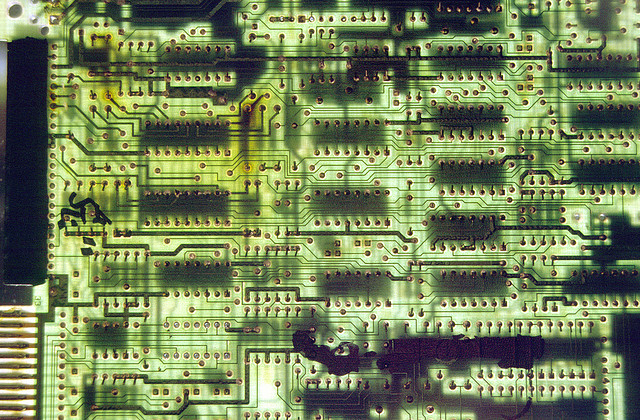
\includegraphics[width=.7\linewidth]{img/electric_city.jpg}\label{img:electric:city}}
\end{frame}
%%%%%%%%%%%%%%%%%%%%%%%%%%%%%%%%%%%%%%%%%%%%%%%%%%%%%%%%%%%%%%%%%%%%%%%%%%%%%%%%%%%%%%%%%
%%%%%%%%%%%%%%%%%%%%%%%%%%%%%%%%%%%%%%%%%%%%%%%%%%%%%%%%%%%%%%%%%%%%%%%%%%%%%%%%%%%%%%%%%
%%%%%%%%%%%%%%%%%%%%%%%%%%%%%%%%%%%%%%%%%%%%%%%%%%%%%%%%%%%%%%%%%%%%%%%%%%%%%%%%%%%%%%%%%
%%%%%%%%%%%%%%%%%%%%%%%%%%%%%%%%%%%%%%%%%%%%%%%%%%%%%%%%%%%%%%%%%%%%%%%%%%%%%%%%%%%%%%%%%
\begin{frame}{Le coin de l'animateur\\[-5pt]
\label{coin::animateur}
  {\large Trucs et astuces pour s'assurer que le message passe bien}}
  \begin{block}{Remarques générales}
    \begin{itemize}
    \item Il faut vous approprier les activités. N'hésitez pas à ne pas suivre
      les consignes à la lettre.\\
      Ces activités sont des bases de discussion avec les participants, il n'y
      a pas d'évaluation à la fin.
    \item Une question récurrente des participants est de savoir ce que
      l'animateur fait, en recherche.\\
      Pensez à préparer une présentation compréhensible de vos recherches, avec
      le domaine général, ses difficultés et applications et quelques mots de
      vos préoccupations propres.\\
      {\footnotesize Exemple: Le domaine de mon travail est le parallélisme:
        est ce que ranger sa chambre va plus vite à 2 ou 3? oui. à 3000? Non,
        on perd du temps à se coordonner. Et pourtant, la météo de demain est
        calculée en utilisant plusieurs milliers d'ordis en même temps, ce qui
        est difficile. Dans ce domaine, mon travail à moi est d'établir des
        instruments scientifiques (simulateurs ou parcs de machines),
        comparables aux télescopes ou microscopes des physiciens, et qui
        servent d'outils aux scientifiques du domaine.}
    \end{itemize}
  \end{block}
  \begin{block}{À propos du mot d'introduction}
    \begin{itemize}
    \item On peut faire cette présentation soit au début, soit juste après
      l'activité sur le jeu de Nim.
    \item Commencer directement par un petit jeu permet d'éviter que les
      participants ne décrochent avant même qu'on ne commence.
    \end{itemize}
  \end{block}
  \begin{block}{À propos du jeu de Nim}
    \begin{itemize}
    \item L'objectif de cette activité est simplement d'introduire la notion d'algorithme
    \item On propose le jeu avec le participant, mais sans dire trop vite qu'on
      a un truc. S'il y a plusieurs participants, on jouera avec plusieurs
      personnes, pour laisser sa chance à chacun. On peut faire une sorte de
      petit tournois.
    \item Il faut bien sûr laisser commencer le participant pour gagner à coup
      sûr. S'il insiste pour ne pas commencer, on peut le faire (et rattraper
      la stratégie gagnante à la première erreur du participant)
    \item On n'introduit l'existence du truc pour gagner que plus tard, quand
      on gagne à plate couture
    \item Si on perd, c'est à dire si on n'a pas réussi à appliquer la
      stratégie gagnante, il faut proposer un match en 3 (ou en 5 en cas de
      coup dur ;)
    \item On peut amener le participant à découvrir la stratégie gagnante en
      groupant les clous par paquets de 4 au lieu de la disposition pyramidale.
    \item Si l'un des participants connaît déjà la stratégie gagnante du jeu,
      il peut remplacer l'animateur dans une partie avec d'autres participants
    \end{itemize}
  \end{block}
\end{frame}

\begin{frame}{Le coin de l'animateur\\[-5pt]
  {\large Trucs et astuces pour s'assurer que le message passe bien}}
  \begin{block}{À propos du jeu du crêpier psycho-rigide}
    \begin{itemize}
    \item L'objectif de cette activité est de trouver un algorithme et de
    le faire verbaliser par les participants
    \item On propose au participant de d'abord tenter de le résoudre
    intuitivement, sans réfléchir
    \item Si le participant bloque, on peut lui donner un conseil : \og~Une
    bonne première étape est de se débrouiller pour mettre la grande en bas~\fg
    \item Si le participant bloque toujours, on peut lui donner un second
    conseil : \og~où est-ce que la grande devrait être pour pouvoir la mettre en
    bas ? ~\fg puis le guider pour l'étape suivante.
    \item On essaie ensuite de faire expliquer l'algorithme par le participant.
    On gagne à ce que ce soit le participant et non l'animateur qui explique aux
    autres, avec ses propres mots.
    \end{itemize}
  \end{block}
%\url{http://interstices.info/jcms/n_52318/genese-dun-algorithme?hlText=cr\%C3\%A8pes}
\end{frame}

\begin{frame}{Le coin de l'animateur\\[-5pt]
  {\large Trucs et astuces pour s'assurer que le message passe bien}}
  \begin{block}{À propos du base-ball multicolore}
    \begin{itemize}
    \item L'objectif de cette activité est d'introduire les notions de
      correction et performances d'algorithmes
    \item Il faut laisser les participants chercher un peu en les faisant verbaliser
    \item S'ils sont sur le point de trouver l'algo juste, on introduit très
      vite l'algo faux pour préserver un enchaînement logique: "oui, ok, mais
      je vais vous montrer une façon de faire rigolote"
    \item Quand l'algo juste est établi, et avant de parler de performance, on
      peut appliquer sur une variante:\vspace{-\baselineskip}
      \begin{itemize}
      \item Chaque participant prend une couleur (une maison placée au sol entre ses pieds)
      \item Chaque participant (sauf 1) prend un bonhomme dans chaque main
      \item À chaque étape, celui qui a une main libre prend un bonhomme dans la main d'un voisin
      \item (attention, c'est fastidieux à 8 ou 9 couleurs, il vaut mieux faire
        deux rondes car l'algo semble $O(n^2)$)
      \end{itemize}
    \item Expérimentalement, l'algo qui tourne converge très souvent vers la
      solution à 5 maisons, mais converge souvent vers la boucle infinie quand
      il y a plus de couleurs. Ne tentez pas le diable ;)
    \item Dans la disposition linéaire, il est plus simple de mettre la couleur
      avec un seul bonhomme à une extrémité, et commencer par remplir la maison
      de l'autre extrémité. Sinon, on se retrouve avec une maison remplie de un
      seul au milieu, et il faut comprendre que la solution passe par le
      stockage temporaire d'un pion de la maison d'à coté sur le trou.
    \item Le discours sur le $O(n)$ est volontairement approximatif. On veut
      faire sentir les choses; faire un vrai cours prend une douzaine d'heures
      (cf. \url{http://www.loria.fr/~quinson/Teaching/TOP/}).
    \item Il serait intéressant de prouver effectivement la correction de
      l'algorithme linéaire, ainsi que de quantifier la probabilité de
      fonctionner de l'algo qui tourne en fonction du nombre de maisons
    \item Au passage, le crépier ne ressemble pas du tout aux tours de Hanoï:
      l'histoire ressemble un peu, mais la résolution est très différente (il y
      a $2^n-1$ étapes à Hanoï et $3\times n$ au crépier\ldots)
    \end{itemize}
  \end{block}
\end{frame}
\end{document}
